\section{Object Detection}
\label{sec:det}
The object detection part of the project consists of feature extraction and triangulation. For the robot to effectively avoid the obstacle and to plan the path accordingly, it has to know the position and orientation of the obstacle. In order to make it simple for implementation, the obstacle selected here for detection is a sphere, which makes the orientation of the obstacle unnecessary. So, the position of the sphere (x,y,z) with respect to the base frame of the robot is enough to avoid it. The feature of the obstacle is further constrained by colour, which is chosen to be red. Since the depth information is critical for the object avoidance, stereo cameras are used. Prior to using the stereo camera, it has to be calibrated accordingly. The stereo camera gives us two images of the same scene, which is essential to get the depth information. More information about the calibration process can be found in the section \ref{sec:calib} of the report.\\

The feature extraction part deals with identifying the obstacle in the 2D image frames from the stereo camera. The result of the feature extraction process is the pixel location (u,v) of the obstacle's centre (the sphere's centre) for both the left and right images of the same scene. The process is continuous and results in the same for each frame from the stereo camera.\\

The triangulation part deals with finding the position of the obstacle (x,y,z) with respect to the camera frame, making use of the intrinsic and extrinsic parameters of the stereo camera. A transformation from the camera frame to the robot's base frame will give us the position of the obstacle in the base frame.

\subsection{Feature Extraction}
\label{sec:feat}

The feature extraction process is based in color segmentation. To get results good enough, this is done in HSV space. The reason to do so is that, in HSV space, color information is separated from brightness information. In that way, we can easily threshold the image according to red color Hue values, abstracting from illumination issues, allowing only the red pixels. The resultant binary image may contain some noisy white pixels, which are eliminated by performing an opening morphological operation with an elliptical kernel. As a result of this operation, we get a binary image with white pixels only for the red ball.\\

The approach is kept as simple as possible, in order to have very low run-times. The workspace of the robot is constant, and the ball is made of a color in high contrast with everything inside it. Color segmentation is enough to provide an accurate detection. With the binary image already working, the next step is to decide which features will be used to feed the system with a point pixel of coordinates locating the ball. The main idea is to approximate its center. To do that, we find the contour of the ball's blob in the image and calculate the minimum circle that encloses that contour. This circle's center is the coordinate that the detector sends to the next phase in the vision system.\\

In figure \ref{fig:feature_extraction}, the sequence of the detection process is shown, from the starting input image to the final detection of the ball.

\begin{figure}[ht!]
\begin{subfigure}{.5\textwidth}
  \centering
  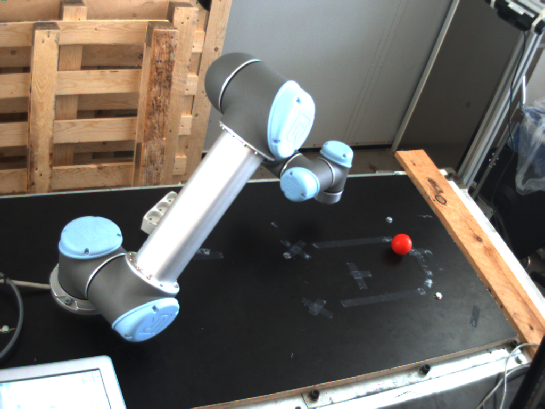
\includegraphics[width=.8\linewidth]{Images/left.png}
  \caption{Original Image Left}
  \label{fig:sfig1}
\end{subfigure}
\begin{subfigure}{.5\textwidth}
  \centering
  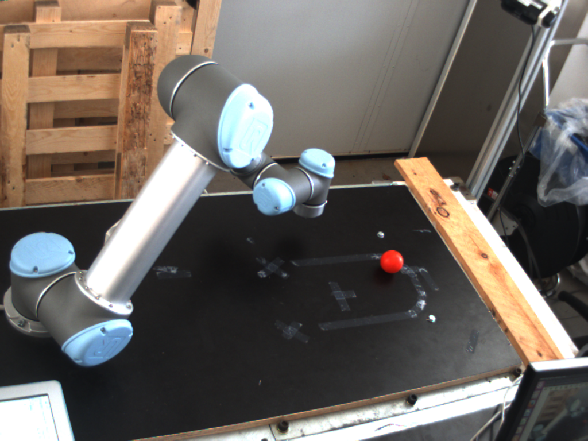
\includegraphics[width=.8\linewidth]{Images/right.png}
  \caption{Original Image Right}
  \label{fig:sfig2}
\end{subfigure}
\begin{subfigure}{.5\textwidth}
  \centering
  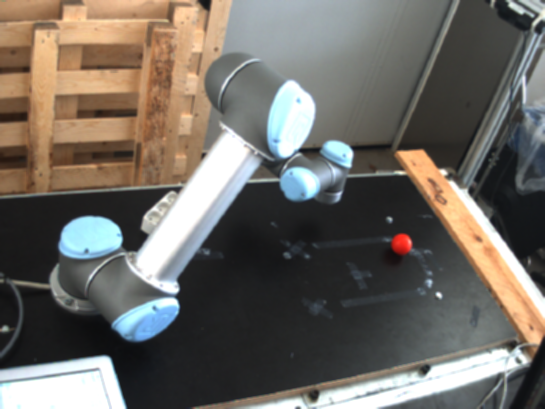
\includegraphics[width=.8\linewidth]{Images/blurred_left.png}
  \caption{Blurred Image Left}
  \label{fig:sfig3}
\end{subfigure}
\begin{subfigure}{.5\textwidth}
  \centering
  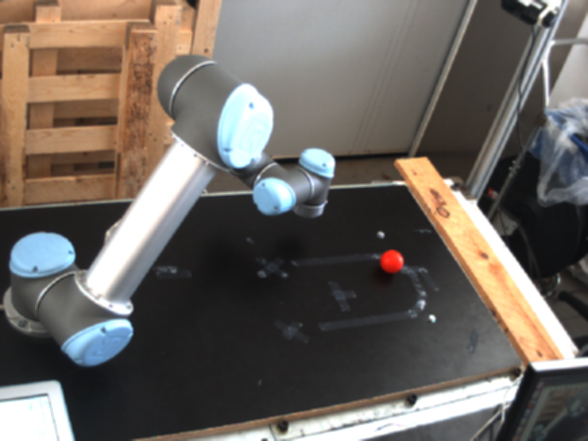
\includegraphics[width=.8\linewidth]{Images/blurred_right.png}
  \caption{Blurred Image Right}
  \label{fig:sfig4}
\end{subfigure}
\begin{subfigure}{.5\textwidth}
  \centering
  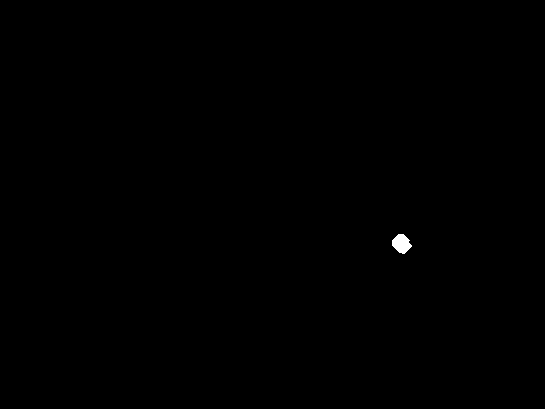
\includegraphics[width=.8\linewidth]{Images/morphed_left.png}
  \caption{Morphed Image Left}
  \label{fig:sfig5}
\end{subfigure}
\begin{subfigure}{.5\textwidth}
  \centering
  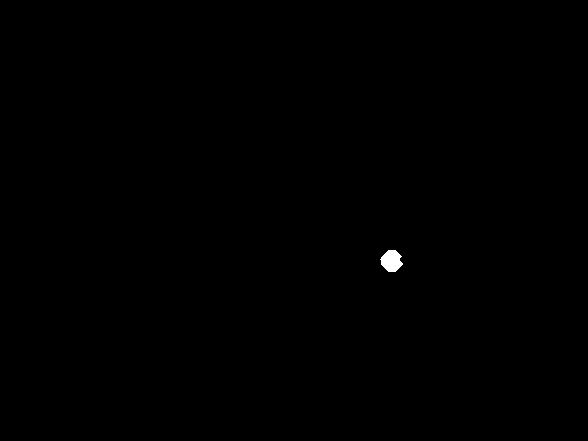
\includegraphics[width=.8\linewidth]{Images/morphed_right.png}
  \caption{Morphed Image Right}
  \label{fig:sfig6}
\end{subfigure}
\begin{subfigure}{.5\textwidth}
  \centering
  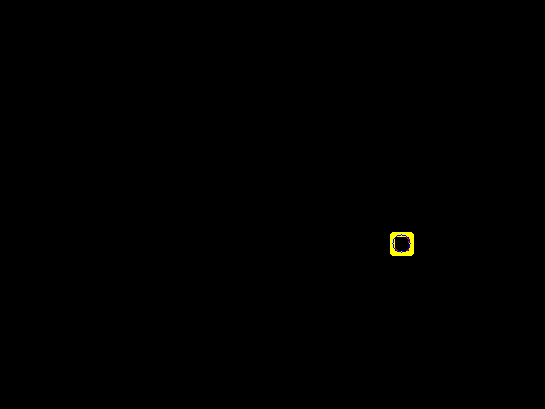
\includegraphics[width=.8\linewidth]{Images/bigbbox_left.png}
  \caption{Bounding Box Left}
  \label{fig:sfig7}
\end{subfigure}
\begin{subfigure}{.5\textwidth}
  \centering
  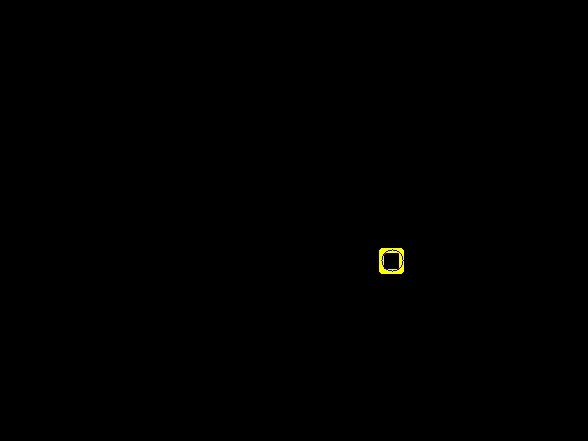
\includegraphics[width=.8\linewidth]{Images/bigbbox_right.png}
  \caption{Bounding Box Right}
  \label{fig:sfig8}
\end{subfigure}
\caption{Resultant images of the feature extraction process}
\label{fig:feature_extraction}
\end{figure}
